\section{VL15}
\textbf{GWAS Aufgaben}
\begin{itemize}
	\item Assoziationstests
	\begin{itemize}
		\item Einzel-SNP, verschiedene genetische Modelle
		\item Scoring-Tests
		\item Haplotypbasierte Analysen, Fine-Mapping
		\item Metaanalyse
		\item SNPxSNP, SNPxKovariablen Interaktionen
		\item Subgruppenanalysen (Power-Problem)
	\end{itemize}
	\item Post-Analyse QC
	\item Graphische Aufbereitung
	\item Extraktion von Kandidaten
	\item Replikation
	\item Vergleich mit Online Ressourcen
\end{itemize}

\subsection{Pedigree Format}
\begin{itemize}
	\item Jede Zeile ein Individuum
	\item Vier IDs: Familie, Individuum, Vater, Mutter
	\item Vater, Mutter – ID muß als Individuum-ID auftreten (0 = fehlend)
	\item Pro SNP zwei Spalten (Allele)
	\item Datenformat erforderlich für viele Softwarepakete
	\item (Gewisse) Familienstruktur ist mit gegeben
\end{itemize}

\subsection{Manhattan Plots}
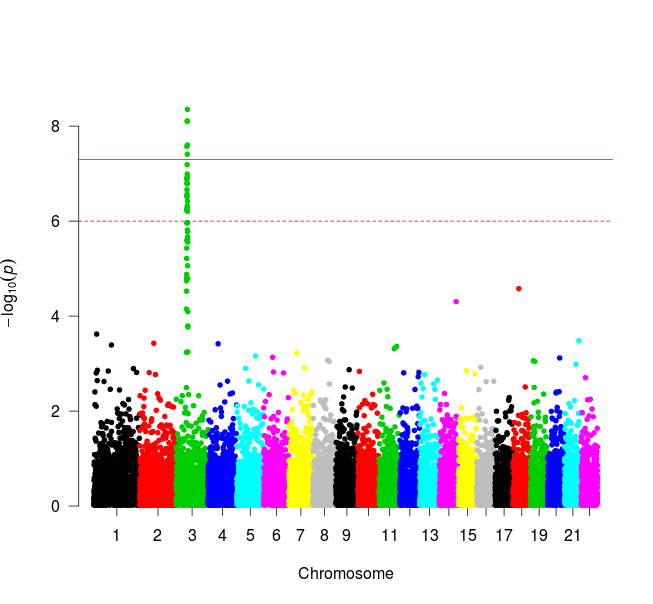
\includegraphics[width=0.5\textwidth]{lectures/V15/pix/manhatten_plot.png}\\
Suggestive-Grenze=$10^{-6}$\\
Genomweite Grenze=$5\cdot 10^{-8}$
\subsection{QQ-Plots}
Idee: Die Mehrzahl der SNPs sollte nicht assoziiert sein, d.h. einer Nullverteilung entsprechen\\
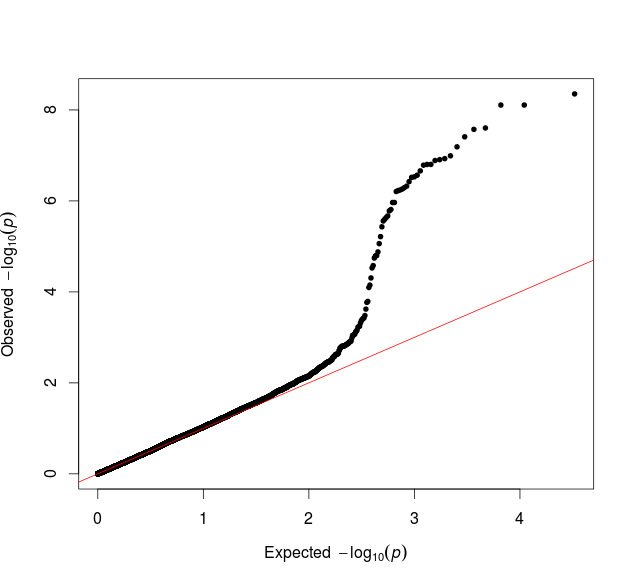
\includegraphics[width=0.5\textwidth]{lectures/V15/pix/qq_plot.png}\\
Wenn Punkte der Mittellinie bis zur Mitte folgen $\rightarrow$ Inflation der Teststatistiken
$\rightarrow$ erfordert Korrektur\\

\underline{Genomic Control:}\\
Inflationsfaktor $\lambda$ berechnen, wenn $\lambda <$ 1.05 $\rightarrow$ keine Korrektur notwendig $\Rightarrow$ siehe \textbf{Genomic Control}

\newpage
\subsection{Regional Association plot (RA)}
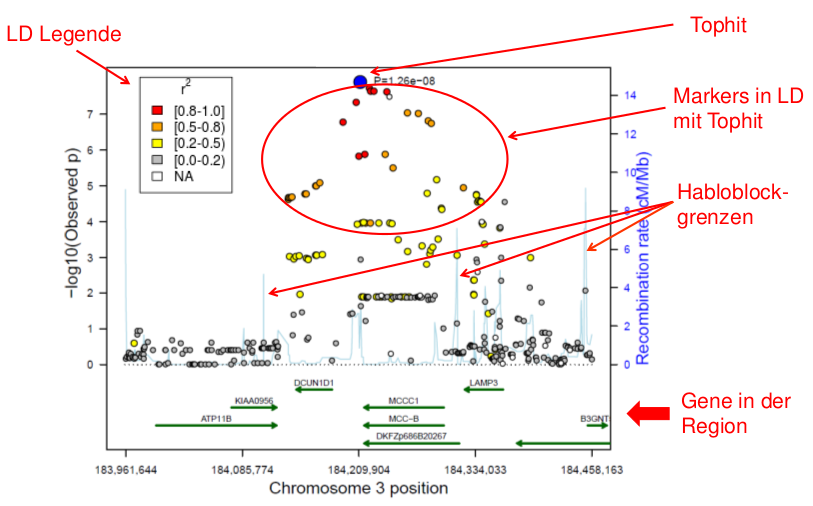
\includegraphics[width=1.0\textwidth]{lectures/V15/pix/ra_plot.png}\\
\textcolor{red}{Was kann man hier so ablesen?}

\subsection{Genomic Control}
Seien $Y_1^2$,…,$Y_m^2$ unabhängige, Chi-Quadrat-verteilte Zufallsvariablen (z.B. aus Fall-Kontrolltests, m = Anzahl Marker)\\\\
Unter H0 (keine Assoziationen) gilt: median($\tilde{Y}_1^2$,…,$\tilde{Y}_m^2$)=0,456\\
Definiere Inflationsfaktor: $\lambda=\frac{\text{median}(Y_1^2\text{,...,}Y_m^2)}{0,456}$\\
Korrigiere Teststatistiken: $(\bar{Y}_1^2\text{,...,}\bar{Y}_m^2) = \frac{Y_1^2\text{,...,}Y_m^2}{\lambda}$\\
\textcolor{red}{Wie kommt man von p-Werten zu Chi-Quadrat-verteilte Zufallsvariablen?}